%%=============================================================================
%% frameworkpoc
%%=============================================================================

\chapter{\IfLanguageName{dutch}{Framework en PoC}{Framework en PoC}}%
\label{ch:frameworkpoc}


Het grootste deel van mijn bachelorproef bestaat uit het opstellen van een competentie framework en bijhorende Proof of concept.

In het volgende deel wordt beschreven hoe het framework is opgesteld en met welke criteria deze beslissingen zijn genomen.
Vervolgens wordt de structuur van de proof of concept samen met de verschillende hoofdstukken overlopen en wordt uitgelegd welke technieken gebruikt zijn voor het realiseren van deze leersite. 
Het doel van dit hoofdstuk is dus tweeledig, enerzijds wordt aangetoond hoe het framework tot stand is gekomen.
Anderzijds wordt uitgelegd hoe het framework omgezet werd naar een praktisch leerplatform dat gebruikt kan worden om het basisniveau 1 van PL/1 en CICS development op IBM Z aan te leren.

\section{Structuur en opbouw van het framework}%
\label{sec:opbouw-van-het-framework}

Qua structuur leunt het competentieframework op gevestigde IBM frameworks, waaronder het IBM z/OS System Administrator Level 1 framework \cite{ibm_z_sysadmin_level1}. 
Deze structuur garandeert een overzichtelijk document dat intuïtief in gebruik is voor zowel studenten als begeleiders in het werkveld.
Het doel is een duidelijk profiel te schetsen van de vereiste junior kennis. 
Het framework is dan niet simpelweg een lijst met onderwerpen, maar een concrete opsomming van eindtermen na het afronden van de leerstof.

Om dit te realiseren is gekozen voor een opbouw met vier vaste pijlers:

\begin{itemize}
    \item \textbf{Het domein:} het specifieke domein waartoe de competentie behoort.
    \item \textbf{De competentie:} het specifieke onderwerp of de vaardigheid die aangeleerd moet worden.
    \item \textbf{De leerdoelen:} de concrete en meetbare acties die aantonen wat de gebruiker begrijpt of kan toepassen.
    \item \textbf{De bronnen:} de literatuur en documentatie die gebruikt zijn om de competentie inhoudelijk te onderbouwen.
\end{itemize}


Aan de hand van deze structuur kan een overzichtelijk document opgesteld worden dat als basis kan dienen voor een proof of concept.
Elke competentie wordt gekoppeld aan concrete leerdoelen zodat duidelijk is welke kennis verwacht wordt.
Hierdoor is het framework niet enkel theoretisch maar ook praktisch toepasbaar.

\section{Criteria voor het bepalen van de competenties}
\label{sec:criteria-bepalen-competenties}

De competenties binnen het framework zijn bepaald aan de hand van meerdere criteria. 
Op deze manier sluit het framework zo goed mogelijk aan bij de kennis die een beginnende PL/1 en CICS developer nodig heeft.
Het Competentieframework PL/1 / CICS developer op z/OS level 1 vertrekt vanuit volgende punten.

\subsection{Basiskennis mainframe}
\label{sec:Basiskennis-mainframeontwikkeling}

Een eerste criterium is de basiskennis die nodig is om mainframeontwikkeling te begrijpen.
Iemand die nog niet vertrouwd is met Z systems moet eerst enkele belangrijke begrippen begrijpen zoals z/OS, PL/1, CICS, datasets, jobs en batch/online transactieverwerking.
Zonder deze basis is het moeilijk om de aangeleerde PL/1 en CICS kennis juist te kunnen plaatsen binnen de ontwikkelingsomgeving.

\subsection{Basis programmeerkennis}
\label{sec:Basiskennis-programmeerkennis}

Een tweede criterium is het bezitten van een basis in programmeerkennis.
Het gebruik van lussen, variabelen en datatypes zijn concepten die aan de basis liggen van elke programmeertaal, hierdoor is het heel waardevol om deze te beheersen voor het programmeren met PL/1 en CICS.

\subsection{Praktijk gericht}
\label{sec:Praktijk-gericht}

Een derde criterium is een sterke focus op de praktijk.
Het framework is bewust niet puur theoretisch ingestoken.
Er is juist veel aandacht voor de daadwerkelijke vaardigheden die op de werkvloer nodig zijn, zoals het efficiënt kunnen lezen en veilig aanpassen van bestaande legacy code.

\subsection{De link met CICS}
\label{sec:link-met-cics}

Een vierde criterium is de integratie met CICS.
Voor online transactieverwerking op mainframes wordt PL/I zelden geïsoleerd gebruikt, maar vrijwel altijd in combinatie met CICS.
Daarom moeten concepten zoals transacties, tasks en datadoorgave via een COMMAREA of channels direct meegenomen worden in de basisopleiding.

\subsection{Hedendaagse IT landschap}
\label{sec:Hedendaagse-IT-landschap}

Een laatste criterium is de connectie met het hedendaagse IT-landschap.
Legacysystemen zoals IBM mainframes opereren binnen een groter geheel.
Om te begrijpen waarom deze talen vandaag de dag nog steeds cruciaal zijn voor grote ondernemingen,
 moet er in het framework ook aandacht zijn voor modernisering en de manier waarop PL/1 en CICS toepassingen integreren met moderne architecturen.


\section{Nodige Competenties}%
\label{sec:Nodige-Competenties}

Aan de hand van de interviews en literatuurstudie is bepaald dat het competentieframework bestaat uit dertien kerncompetenties.
Deze zijn gegroepeerd in vijf categorieën die samen de basis vormen voor een Level 1 developer:

\begin{itemize}
    \item \textbf{Fundamenten en Systeemcontext (Competentie 1-2):} Omvat algemene programmeerlogica en IBM Z basiskennis. Deze zijn noodzakelijk om de technische omgeving en de werking van het mainframe ecosysteem te begrijpen voordat specifieke talen worden aangeleerd.
    
    \item \textbf{PL/I Taalbeheersing (Competentie 3-4):} Behandelt de theoretische syntax en de praktische toepassing van PL/I. Dit is essentieel omdat PL/I de primaire programmeertaal is waarin de bedrijfslogica geschreven wordt.
    
    \item \textbf{CICS Transactieverwerking (Competentie 5-7):} Richt zich op CICS concepten en de integratie hiervan in PL/1 programma's. Dit is onmisbaar voor het ontwikkelen en begrijpen van onlinetransactiesystemen op de mainframe.
    
    \item \textbf{Buildprocessen en Foutafhandeling (Competentie 8-10):} Behandelt de buildflow, JCL basis en systematische troubleshooting. Deze kennis is nodig om code succesvol te compileren en bugs te verhelpen.
    
    \item \textbf{Bedrijfscontext en Onderhoud (Competentie 11-13):} Focust op codeanalyse, de historische context en modernisering. Dit is cruciaal om de blijvende waarde van legacysystemen te begrijpen en ze veilig te kunnen onderhouden binnen moderne IT architecturen.
\end{itemize}

Het gemaakte framework vormt hiermee de inhoudelijke blauwdruk voor de leerstof, waarbij de dertien competenties de basis leggen voor het praktische gedeelte van deze proef.
\section{Volgende niveau Competenties}%
\label{sec:Volgende-Competenties}

Bewust is gekozen voor een scherpe afbakening op een basisniveau of junior profiel, dit waarborgt een haalbare leercurve.
De overgang naar een volgend niveau aangeduid als Level 2 of medior profiel markeert de stap van conceptuele kennis naar praktische complexe applicatieontwikkeling.
Waar niveau 1 zich richt op de oriëntatie binnen het ecosysteem en het uitvoeren van kleine aanpassingen, vereist niveau 2 dat een developer zelfstandig volledige programma architecturen kan opzetten en optimaliseren.
De volgende competenties vormen de kern van deze verdieping:


\subsection{Geavanceerde PL1}
\label{sec:geavanceerde-pli}
Op Niveau 1 ligt de focus op de basis van PL/I zoals variabelen en simpele procedures.
Niveau 2 gaat dieper in op het geheugenbeheer, hier leert de ontwikkelaar werken met dynamic storage allocation via pointers en based of controlled variabelen. 
Daarnaast is het op dit niveau essentieel om complexe foutafhandeling te implementeren via ON-units, waardoor applicaties niet simpelweg crashen, maar gecontroleerd kunnen herstellen van runtime fouten.
Dit zorgt voor de robuustheid die in een enterprise omgeving vereist is.

\subsection{CICS verdieping}
\label{sec:cics-verdieping}
De stap naar Niveau 2 binnen CICS betekent de overgang van het lezen van code naar het bouwen van volledige online applicaties.
Dit omvat de ontwikkeling van gebruikersinterfaces via BMS-maps (Basic Mapping Support) voor 3270-terminals. 
Verder leert de ontwikkelaar hoe hij via File Control rechtstreeks gegevens kan wegschrijven, updaten of verwijderen in VSAM bestanden.
Ook het efficiënt gebruik van Temporary Storage Queues (TSQ) voor tijdelijke dataopslag gedurende een sessie is een cruciaal onderdeel van deze gevorderde kennis.

\subsection{Geavanceerde tooling en diagnostiek}
\label{sec:geavanceerde-tooling}
Waar een junior vaak afhankelijk is van eenvoudige "display" statements of compiler listings voor debugging, maakt een Niveau 2 developer gebruik van gespecialiseerde tools.
Dit omvat het beheersen van de IBM z/OS Debugger om stap voor stap door complexe programmaflows te lopen. 
Daarnaast leert men op dit niveau hoe men systeem dumps moet interpreteren (bijvoorbeeld via IPCS) om de exacte oorzaak van een abend (applicatie crash) in de systeemkern te achterhalen.

\subsection{Performantie optimalisatie en efficiëntie}
\label{sec:performantie-optimalisatie}
In een omgeving waar miljoenen transacties per seconde worden verwerkt, is efficiëntie alles.
Een Niveau 2 developer begrijpt de impact van code op het CPU verbruik. 
Men leert technieken om I/O operaties te minimaliseren en SQL queries of CICS commando's te tunen. 
De focus verschuift hier van "de code werkt" naar "de code werkt met een minimale footprint".

\subsection{Security architectuur}
\label{sec:security-architectuur}
Beveiliging op Niveau 2 gaat verder dan het simpelweg hebben van een inlogcode.
De ontwikkelaar leert hoe applicatiecode moet integreren met externe security managers zoals RACF.
Dit houdt in dat men begrijpt hoe men autorisatie checks uitvoert binnen de code, zodat gevoelige bedrijfsdata enkel toegankelijk is voor geautoriseerde gebruikers of specifieke transactie ID's.

\subsection{Modernisering}
\label{sec:modernisering-api-integratie}
Niveau 2 slaat de definitieve brug naar moderne IT.
De ontwikkelaar leert hoe hij legacy PL1 en CICS programma's kan verbinden met RESTful API's via z/OS Connect.
Hierdoor kan de ontwikkelaar copybooks (mainframe datastructuren) omzetten naar JSON formaat.
Als resultaat kan legacy backend logica eenvoudig communiceren met moderne web applicaties en mobiele interfaces in een hybride cloud omgeving.


\section{Van framework naar Proof of Concept}
\label{sec:van-framework-naar-proof-of-concept}

Het uitgewerkte framework wordt gebruikt als de functionele blauwdruk voor de proof of concept.
Waar het framework antwoord geeft op de 'wat' vraag (wat moet men kennen?), beantwoordt de PoC de 'hoe' vraag (hoe leer je deze concepten?).
De PoC is gerealiseerd als een laagdrempelige leersite die de student begeleidt in het verwerven van de gedefinieerde competenties.

Door de chronologie van het framework te respecteren en eerst universele logica te behandelen, dan de taal, gevolgd door debugging en context, wordt het brengen van te moeilijke leerstof vermeden.
Dit verlaagt de drempel aanzienlijk voor IT'ers die nog nooit met een mainframe in contact zijn gekomen.

\section{Structuur en opbouw van de PoC leersite}%
\label{sec:opbouw-van-de-leersite}


De leersite is modulair opgebouwd, waarbij elke pagina direct te herleiden is naar één of meerdere leerdoelen uit het opgestelde competentie framework. 
De vaste flow ziet er als volgt uit:

\begin{itemize}
    \item \textbf{Fase 1:} Bepalen nodige technologieën voor ontwikkeling van basis site.
    \item \textbf{Fase 2:} Scope van content bepalen die in de leersite gaan worden opgenomen.
    \item \textbf{Fase 3:} Aan hand van literatuurstudie en interviews relevante inhoud toevoegen.
\end{itemize}

\section{Bepalen van technologieën}%
\label{sec:Bepalen-van-technologien}

In de opstartfase van dit project werd bewust tijd vrijgemaakt om de technologie keuzes af te toetsen aan het doel van de proof of concept.
Het doel van de PoC was een toegankelijke leersite rond PL/1 en CICS met theorie, oefeningen en quizzen die vlot kan uitgebreid worden zonder extra hostingkost.
De keuze ging daarom niet naar de meest exotische of meest enterprise stack, maar naar een set technieken die snel resultaat opleveren en gemakkelijk onderhoudbaar zijn en tegelijk voldoende structuur bieden voor groei.

\subsection{Selectiecriteria}%
\label{sec:Selectiecriteria-technologien}
De technologieën werden beoordeeld op volgende criteria:
\begin{itemize}
  \item \textbf{Flexibiliteit en uitbreidbaarheid}: nieuwe cursussen en onderdelen (theorie, oefening, quiz) moeten toegevoegd kunnen worden zonder ingrijpende code wijzigingen.
  \item \textbf{Vertrouwdheid en leercurve}: de ontwikkeltijd is beperkt dus de stack moest aansluiten bij bestaande webkennis.
  \item \textbf{Kost en deploybaarheid}: aangezien er geen budget is voor hosting, moet de leersite goedkoop publiceerbaar zijn.
  \item \textbf{Performantie en gebruikservaring}: snelle laadtijden en een responsieve interface zijn belangrijk om de leersite aangenaam te gebruiken.
  \item \textbf{Veilig omgaan met leercontent}: leerinhoud bevat opmaak en soms embedded media dat moet veilig weergegeven worden in de browser.
\end{itemize}

\subsection{Gekozen basis van webtechnologieën}%
\label{sec:basis-webtechnologieën}
De proof of concept is een webapplicatie en gebruikt daarom de klassieke web basis: HTML voor structuur, CSS voor styling en JavaScript voor interactiviteit.
Deze keuze sluit aan bij het doelpubliek (leren via een browser, zonder extra installatie) en maakt het mogelijk om de site als statisch pakket te publiceren.

\subsection{React als UI laag}%
\label{sec:React-ui}
Voor de gebruikersinterface werd gekozen voor React.
De leersite bevat meerdere schermen en componenten waaronder cursusoverzichten, hoofdstukken, theoriepagina’s, oefeneditor en quizes waarbij de UI dynamisch mee evolueert met de selectie van de gebruiker.
React maakt het eenvoudiger om zulke herbruikbare componenten op te bouwen en toestand zoals de geselecteerde cursus of het thema consistent te beheren.
Concreet in dit project:
\begin{itemize}
  \item cursussen worden in de interface als kaarten gepresenteerd en leiden naar een detailpagina met hoofdstuknavigatie.
  \item het thema donker en licht wordt opgeslagen in localStorage zodat de voorkeur bewaard blijft.
  \item verschillende onderdelen Theory,Exercise en Quiz delen dezelfde navigatiestructuur en layout wat component hergebruik stimuleert.
\end{itemize}

\subsection{Vite als build en ontwikkeltool}%
\label{sec:vite-build}
Om de ontwikkelervaring snel en efficiënt te houden werd Vite gekozen als buildtool rond React.
Vite staat bekend om snelle lokale ontwikkeling (snelle herlaadtijden en Hot Module Replacement) en levert ook een geoptimaliseerde productie build.
Voor een proof of concept is dit essentieel, de focus blijft op functionaliteit en content zonder onnodige tijd te verliezen aan trage builds of complexe configuratie.
Daarnaast past Vite goed bij het deploy doel, de output kan als statische site worden gehost.

\subsection{Tailwind CSS voor consistente en schaalbare styling}%
\label{sec:Tailwind-styling}
Voor de vormgeving werd Tailwind CSS gebruikt aangevuld met PostCSS en Autoprefixer.
Tailwind ondersteunt een utility first aanpak waarmee de interface snel consistent kan worden opgebouwd, zonder dat een grote hoeveelheid aparte CSS bestanden en naming conventies nodig is.
Dit is nuttig in een leerplatform waar veel herhaalpatronen bestaan (panelen, knoppen, kaarten, navigatie) én waar het ontwerp later nog kan evolueren.
In dit project is ook expliciet gekozen voor dark mode via een class strategie, omdat die aanpak goed werkt met Tailwind en eenvoudig te onderhouden is.

\subsection{Content als JSON eenvoudig uitbreiden met nieuwe cursussen}%
\label{sec:JSON-cursussen}
Een belangrijk ontwerpdoel was uitbreidbaarheid, nieuwe leerinhoud moet toegevoegd kunnen worden zonder telkens React code aan te passen.
Daarom wordt course content per cursus opgeslagen in een index.json bestand met een vaste structuur bestaande uit hoofdstukken, theorie, oefeningen en quizvragen.
Deze aanpak heeft meerdere voordelen:
\begin{itemize}
  \item \textbf{schaalbaar}: nieuwe cursussen of hoofdstukken toevoegen is in grote mate een inhouds taak;
  \item \textbf{versiebeheerbaar}: JSON bestanden zijn ideaal om in Git te beheren en te reviewen;
  \item \textbf{scheiding van verantwoordelijkheden}: UI en content blijven duidelijk gescheiden.
\end{itemize}

\subsection{Markdown en veilige HTML rendering}%
\label{sec:Markdown-rendering}
Voor theorie inhoud wordt waar mogelijk Markdown gebruikt, omdat het laagdrempelig is om te schrijven en leesbaar blijft in bronvorm.
Bij het renderen in de browser wordt Markdown omgezet naar HTML.
Om te vermijden dat content onveilig of ongewenst HTML/JavaScript zou injecteren, wordt de output gefiltert met DOMPurify.
Embedded video’s worden gecontroleerd toegelaten, zodat de leersite veilig blijft terwijl interactieve content toch mogelijk is.

\subsection{Lokale media zonder extra backend}%
\label{sec:Lokale-backend}
De leersite ondersteunt videomateriaal door bestanden in de folder public/videos/ te plaatsen en die via bestandsnaam te refereren in de JSON content.
Dit is een pragmatische keuze voor een proof of concept want er is geen aparte backend of streamingplatform nodig, en toch kan de leerervaring verrijkt worden met videos en afbeeldingen.

\subsection{Waarom geen backend of database?}%
\label{sec:backend-database}
Er is bewust geen server side component toegevoegd in deze fase.
De kern van de proof of concept is het valideren van de leerflow, de contentstructuur en de gebruikerservaring.
Door te kiezen voor een statische front end met JSON content blijft de deploy eenvoudig en kosteloos, en kunnen iteraties snel gebeuren.
Mocht later behoefte ontstaan aan voortgangsopslag of gepersonaliseerde trajecten dan kan er in een volgende fase alsnog een backend worden toegevoegd.

\subsection{Conclusie technologieën}%
\label{sec:Conclusie-technologien}
De uiteindelijke technologie set (React, Vite, Tailwind CSS, JSON content, Markdown met filtering en statische media) sluit nauw aan bij de projectdoelen:
snelle ontwikkeling, lage kost, veilige contentweergave en een structuur die het toevoegen van nieuwe PL1 en CICS leermodules zo eenvoudig mogelijk maakt.


\section{Verschillende modules in de leersite}%
\label{sec:Modules-in-leersite}

De leersite is opgebouwd uit zes modules die samen een volledig en geleidelijk leertraject vormen rond PL/I en CICS. 
Elke module heeft een eigen plaats binnen het traject en werd opgenomen aan de hand van de feedback door professionals.
Hierdoor leren studenten niet alleen afzonderlijke concepten zoals de PL/1 syntax, maar begrijpen ze hoe die in een bredere mainframecontext met elkaar samenhangen en zijn ontstaan.

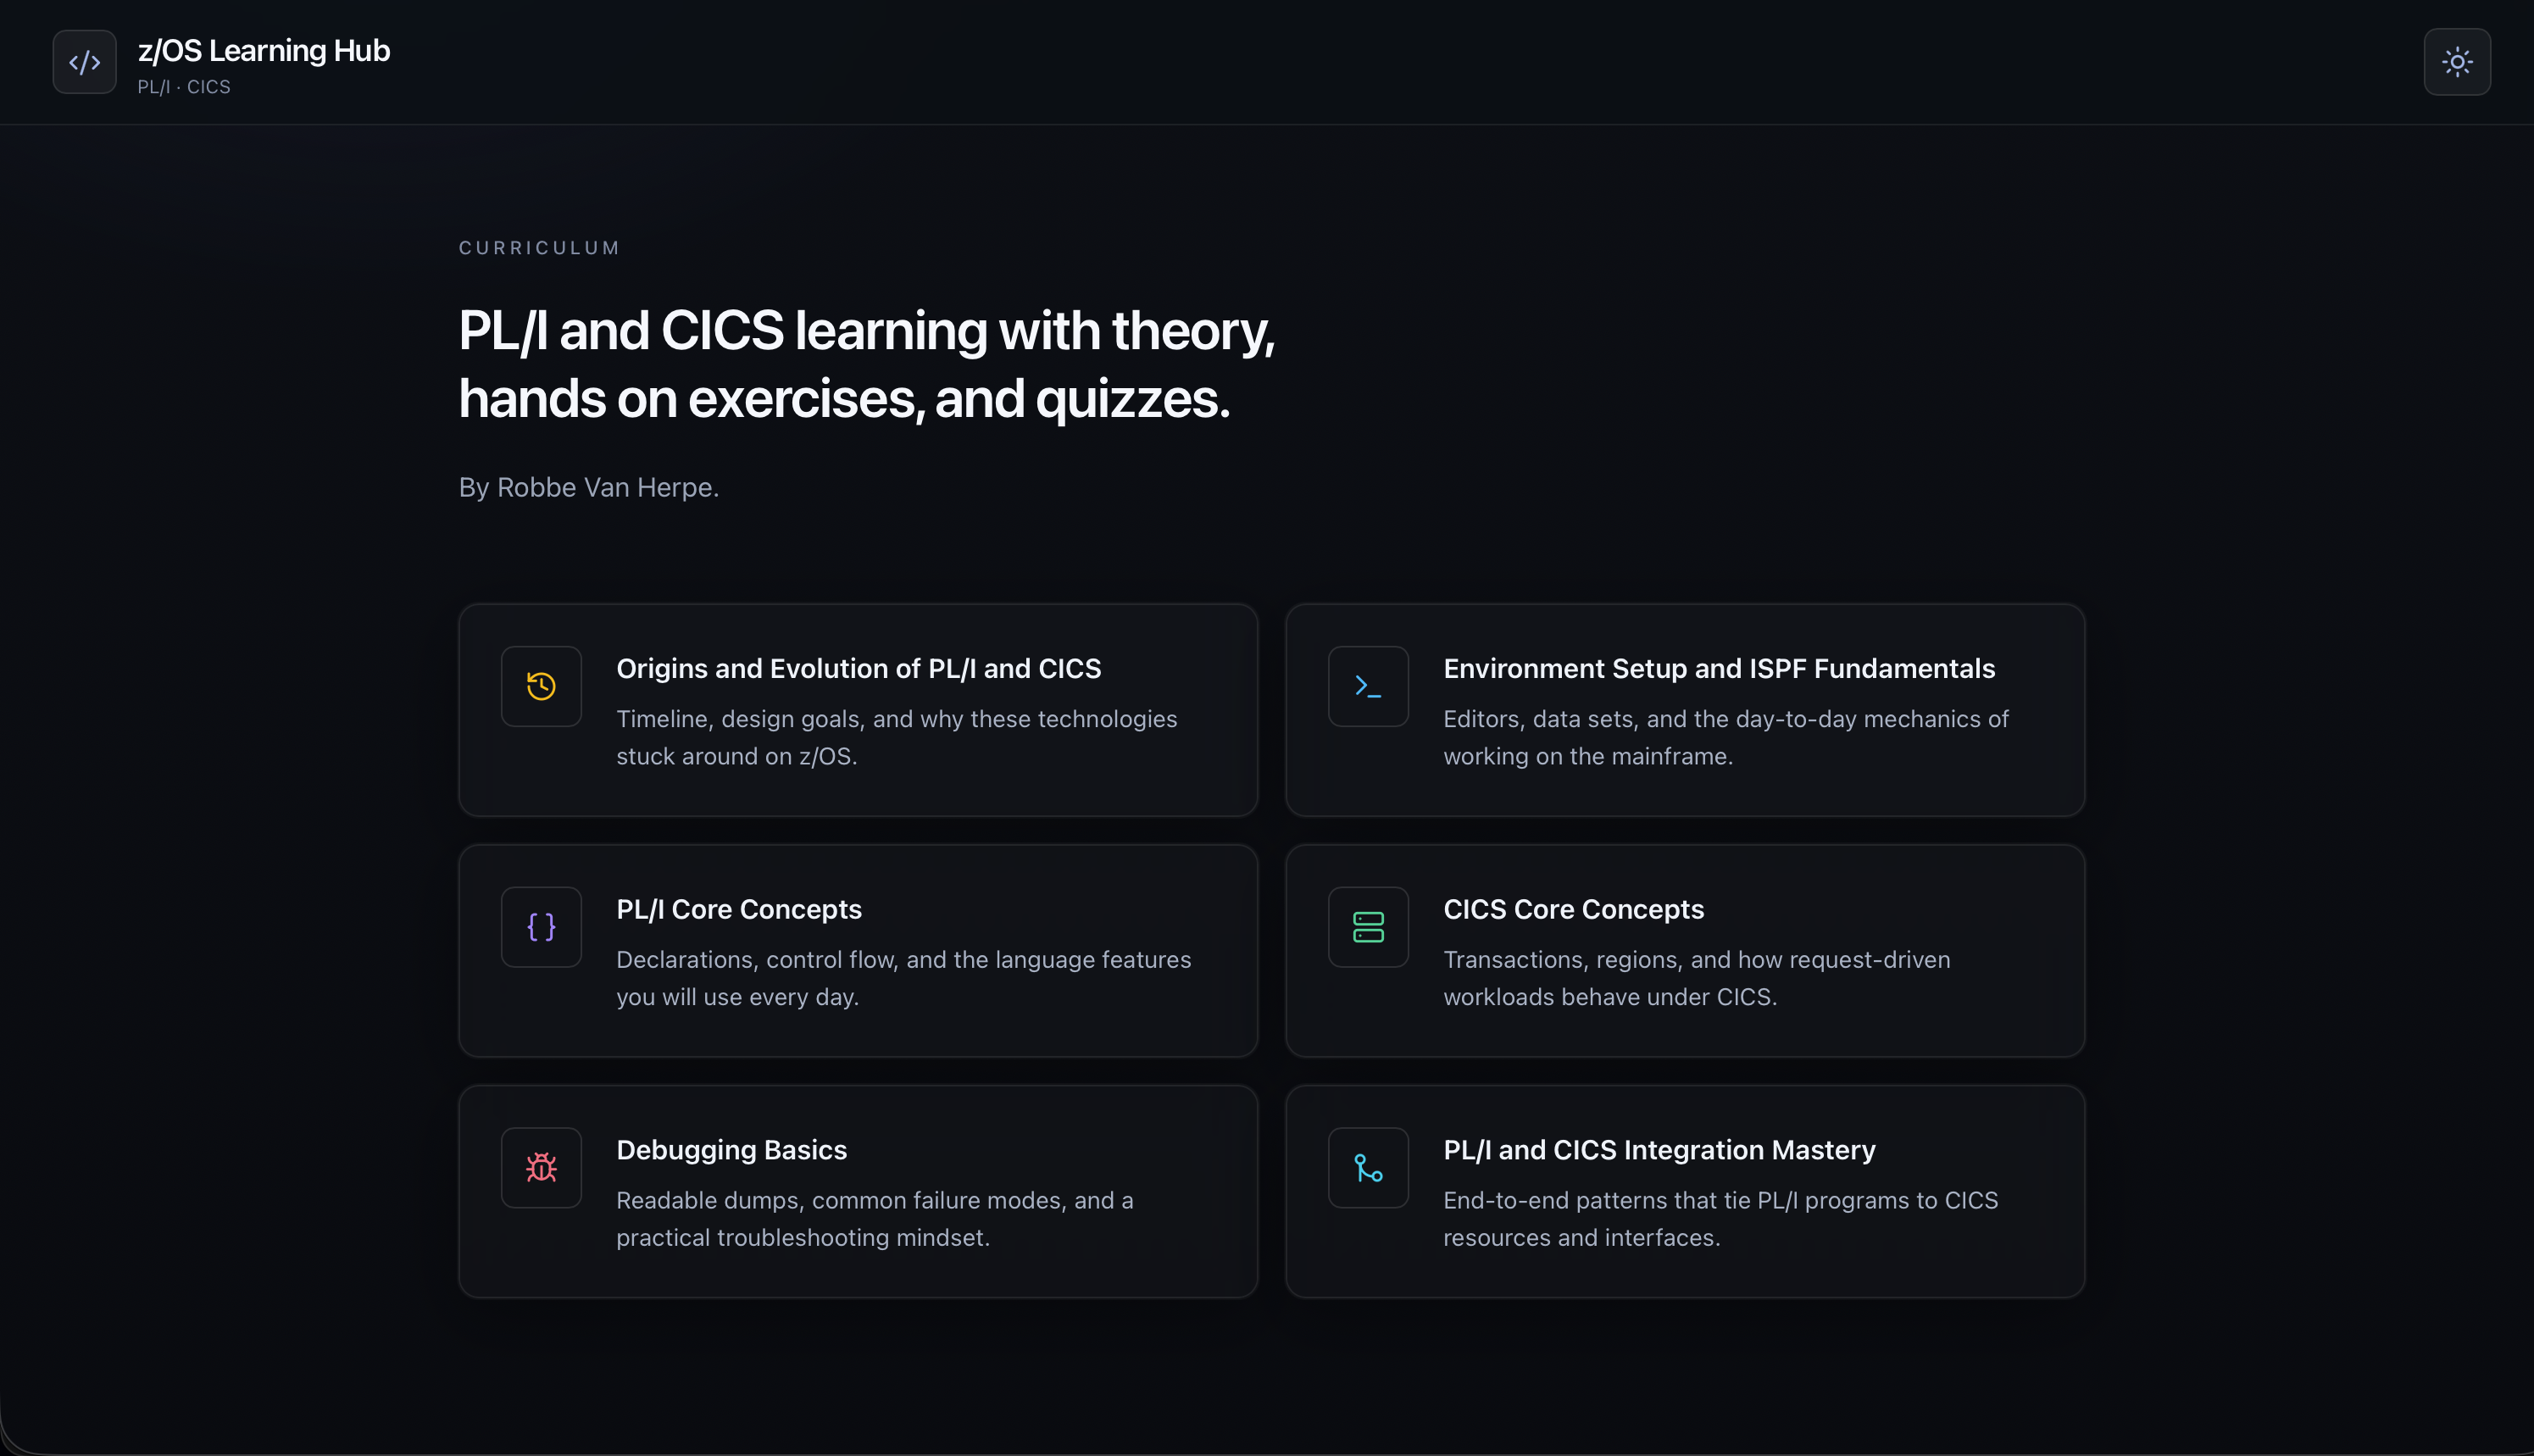
\includegraphics[width=0.45\textwidth]{../graphics/mainscreen.png}

\subsection[short]{Origins and Evolution of PL/I and CICS}%
\label{sec:origins-pl1cics}

De module \textbf{Origins and Evolution of PL/I and CICS} werd opgenomen omdat het belangrijk is dat studenten eerst
 begrijpen waar deze technologieën vandaan komen en waarom ze vandaag nog steeds even relevant zijn. 

Zonder de historische en conceptuele kennis zouden PL/I en CICS kunnen overkomen als irrelevante en eerder verouderde technologieën.
Dit terwijl het net die systemen zijn die voor veel bedrijven nog steeds een zeer cruciale rol spelen binnen de financiële sector.
Door te beginnen met de oorsprong en evolutie van deze technologieën krijgt de student een beter inzicht in hun plaats binnen enterprise computing en de redenen waarom organisaties er nog steeds op vertrouwen voor kritieke toepassingen.

Deze module sluit direct aan op competentie 12.0 (Historische en enterprise-context) en competentie 13.0 (Modernisering en integratie) van het competentieframework.


\subsection[short]{Environment Setup and ISPF Fundamentals}%
\label{sec:Environment-pl1cics}


De module \textbf{Environment Setup and ISPF Fundamentals} legt de praktische basis om te leren werken met ISPF en Zowe Explorer.
Het leren werken met deze code editors behandelt de competentie 2.0 (IBM Z basiskennis) en stelt de student in staat om zijn ontwikkelingsomgeving te beheersen.
De student leert navigeren door schermstructuren en beheert datasets en jobs, wat essentieel is voor een goede start binnen het ecosysteem.

Legacy technologieën zoals ISPF hebben een steile leercurve voor nieuwe developers, daarom wordt er in dit thema ook gefocust op alternatieven zoals Zowe Explorer.
Studenten zijn moderne code editors zoals VSCode gewend en kunnen hierdoor efficiënter werken met deze tools.
Daarom is deze module gefocust op beide manieren om de drempel zo laag mogelijk te maken voor nieuwe ontwikkelaars.
Deze module zou als eindresultaat de student een goede basis moeten geven om te navigeren in hun ontwikkelingsomgeving,
 waardoor ze zich vervolgens kunnen focussen op het leren van PL/1 en CICS.


\subsection[short]{PL/I Core Concepts}%
\label{sec:core-pl1}

De module \textbf{PL/I Core Concepts} vormt de basis voor het programmeergedeelte van de leersite en is daarom cruciaal.
Het behandelt enkele competenties, waaronder competentie 3.0 (PL/I taalbasis) en competentie 4.0 (PL/I programmeerpraktijk).
Daarnaast wordt hier ook competentie 1.0 (Fundamenten in programmeren) opgefrist in een mainframecontext.

Studenten leren de specifieke syntaxis en declaraties van PL/1 samen met de programmastructuren.
Dit zorgt ervoor dat ze niet alleen code leren reproduceren maar ook begrijpen hoe PL/1 logisch is opgebouwd binnen een professionele omgeving.
Deze module vormt de bouwstenen waarop verder gebouwd kan worden om te werken binnen complexe legacysystemen als developer.


\subsection[short]{CICS Core Concepts}%
\label{sec:core-cics}

De module \textbf{CICS Core Concepts} is opgenomen omdat kennis van PL/1 alleen niet volstaat wanneer men wil werken in transactionele mainframesystemen.
CICS is een cruciaal onderdeel van veel bedrijfsapplicaties en bepaalt hoe transacties worden uitgevoerd.
Daarnaast zorgt CICS voor het controleren van gegevensstromen en het verwerken van gebruikersinteracties met het systeem.

Het is dus belangrijk dat de student inzicht krijgt in de werking van CICS als systeemlaag naast het gebruik binnen PL/1 zelf.
De module legt uit wat transacties, tasks en resources zijn zodat de student de noodzakelijke conceptuele basis heeft om later PL/1 programma’s succesvol in een transactionele omgeving te laten draaien.
Hiermee volbrengt deze module competentie 5.0 (CICS concepten).


\subsection[short]{Debugging Basics}%
\label{sec:debug-pl1cics}

De module \textbf{Debugging Basics} is belangrijk omdat leren programmeren of werken met mainframes niet alleen draait om het schrijven van correcte code maar ook om het kunnen herkennen, analyseren en oplossen van fouten.
In deze module leren studenten onderscheid maken tussen de verschillende soorten fouten en maken ze kennis met het gebruik van IBM message manuals.
Door deze eigenschappen kan de module gekoppeld worden aan competentie 10.0 (Foutanalyse en troubleshooting).
In technische opleidingen is debugging een fundamentele vaardigheid, het geeft studenten een beter beeld tijdens het programmeren wanneer ze geconfronteerd worden met een probleem.
Doordat hier een aparte module voor is voorzien zijn studenten beter gewapend tijdens hun eerste weken op de werkvloer wanneer ze zelfstandig problemen moeten oplossen.
Deze module verhoogt dus niet alleen de technische kennis, maar ook het probleemoplossend denken van de student.


\subsection[short]{PL/I and CICS Integration Mastery}%
\label{sec:mastery-pl1cics}

Tot slot is de module \textbf{PL/I and CICS Integration Mastery} opgenomen omdat je met al deze concepten apart niet het volledige totaalbeeld ziet.
Hiervoor is een module nodig die al deze afzonderlijke domeinen samenbrengt tot een meer geavanceerde en realistische context.
Nadat de student inzicht heeft verworven in zowel PL/1 als CICS afzonderlijk, is het noodzakelijk om te tonen hoe beide in de praktijk met elkaar geïntegreerd worden.

Deze module integreert de competenties: 6.0 (CICS programmeerbasis), 7.0 (Gegevensuitwisseling in CICS), 8.0 (Build- en compileflow) en 11.0 (Codeanalyse en onderhoud) om tot één geheel te komen.

Studenten maken hier de overstap naar geavanceerde toepassingen, waarbij ze leren hoe programma’s via de COMMAREA communiceren en hoe een volledige buildflow van translate tot link edit verloopt.
Op deze manier leert de student niet alleen de onderdelen technisch te beheersen, maar ook de totale visie te behouden die nodig is voor professionele applicatieontwikkeling.

Deze module is daarom belangrijk als afsluiting van het leertraject, want studenten leren om de geïsoleerde leerinhouden toe te passen in een meer realistische mainframeomgeving. 

Samen zorgen deze zes modules voor een opbouw die logish en opbouwend is. 

De structuur van het leerplatform begeleidt de gebruiker stapsgewijs: van de initiële introductie en theoretische context, via de technische fundamenten, naar de uiteindelijke praktische implementatie.
Hierdoor ontstaat er een leeromgeving die studenten aanzet om verder te gaan met de theoretische kennis die wordt opgedaan.
Als resultaat bekomen we studenten die de brug kunnen slaan tussen abstracte theorie en de complexe realiteit van een professionele mainframeomgeving, en zo met vertrouwen hun eerste stappen als junior developer kunnen zetten.



\section{Bepalen opbouw van de modules}%
\label{sec:opbouw-van-modules}

Nadat de verschillende modules zijn gekozen is het bepalen van de opbouw van deze onderdelen cruciaal.
Er moet een logische opbouw zijn zodat studenten hun kennis steeds kunnen opbouwen en direct kunnen testen.

De opbouw van elk hoofdstuk binnen de leersite is bewust opgedeeld in drie vaste onderdelen: een theoretisch gedeelte, een oefengedeelte en een afsluitende quiz. 

Deze structuur werd gekozen om de gebruiker stapsgewijs door het leerproces te begeleiden. 
Eerst wordt de nodige kennis aangebracht, vervolgens krijgt de gebruiker de kans om die kennis toe te passen, 
en tot slot wordt nagegaan in welke mate de inhoud daadwerkelijk begrepen en beheerst wordt. 

Op deze manier wordt de student ondersteund bij ieder onderwerp en ervaren ze steeds kleine mini succesjes die hen motiveren doorheen het hele proces.


\subsection[short]{Theorie in modules}%
\label{sec:Theorie-module}

In het eerste onderdeel \textbf{de theorie}, wordt de inhoud van het hoofdstuk uitgebreid toegelicht.

\begin{figure}
   \centering
   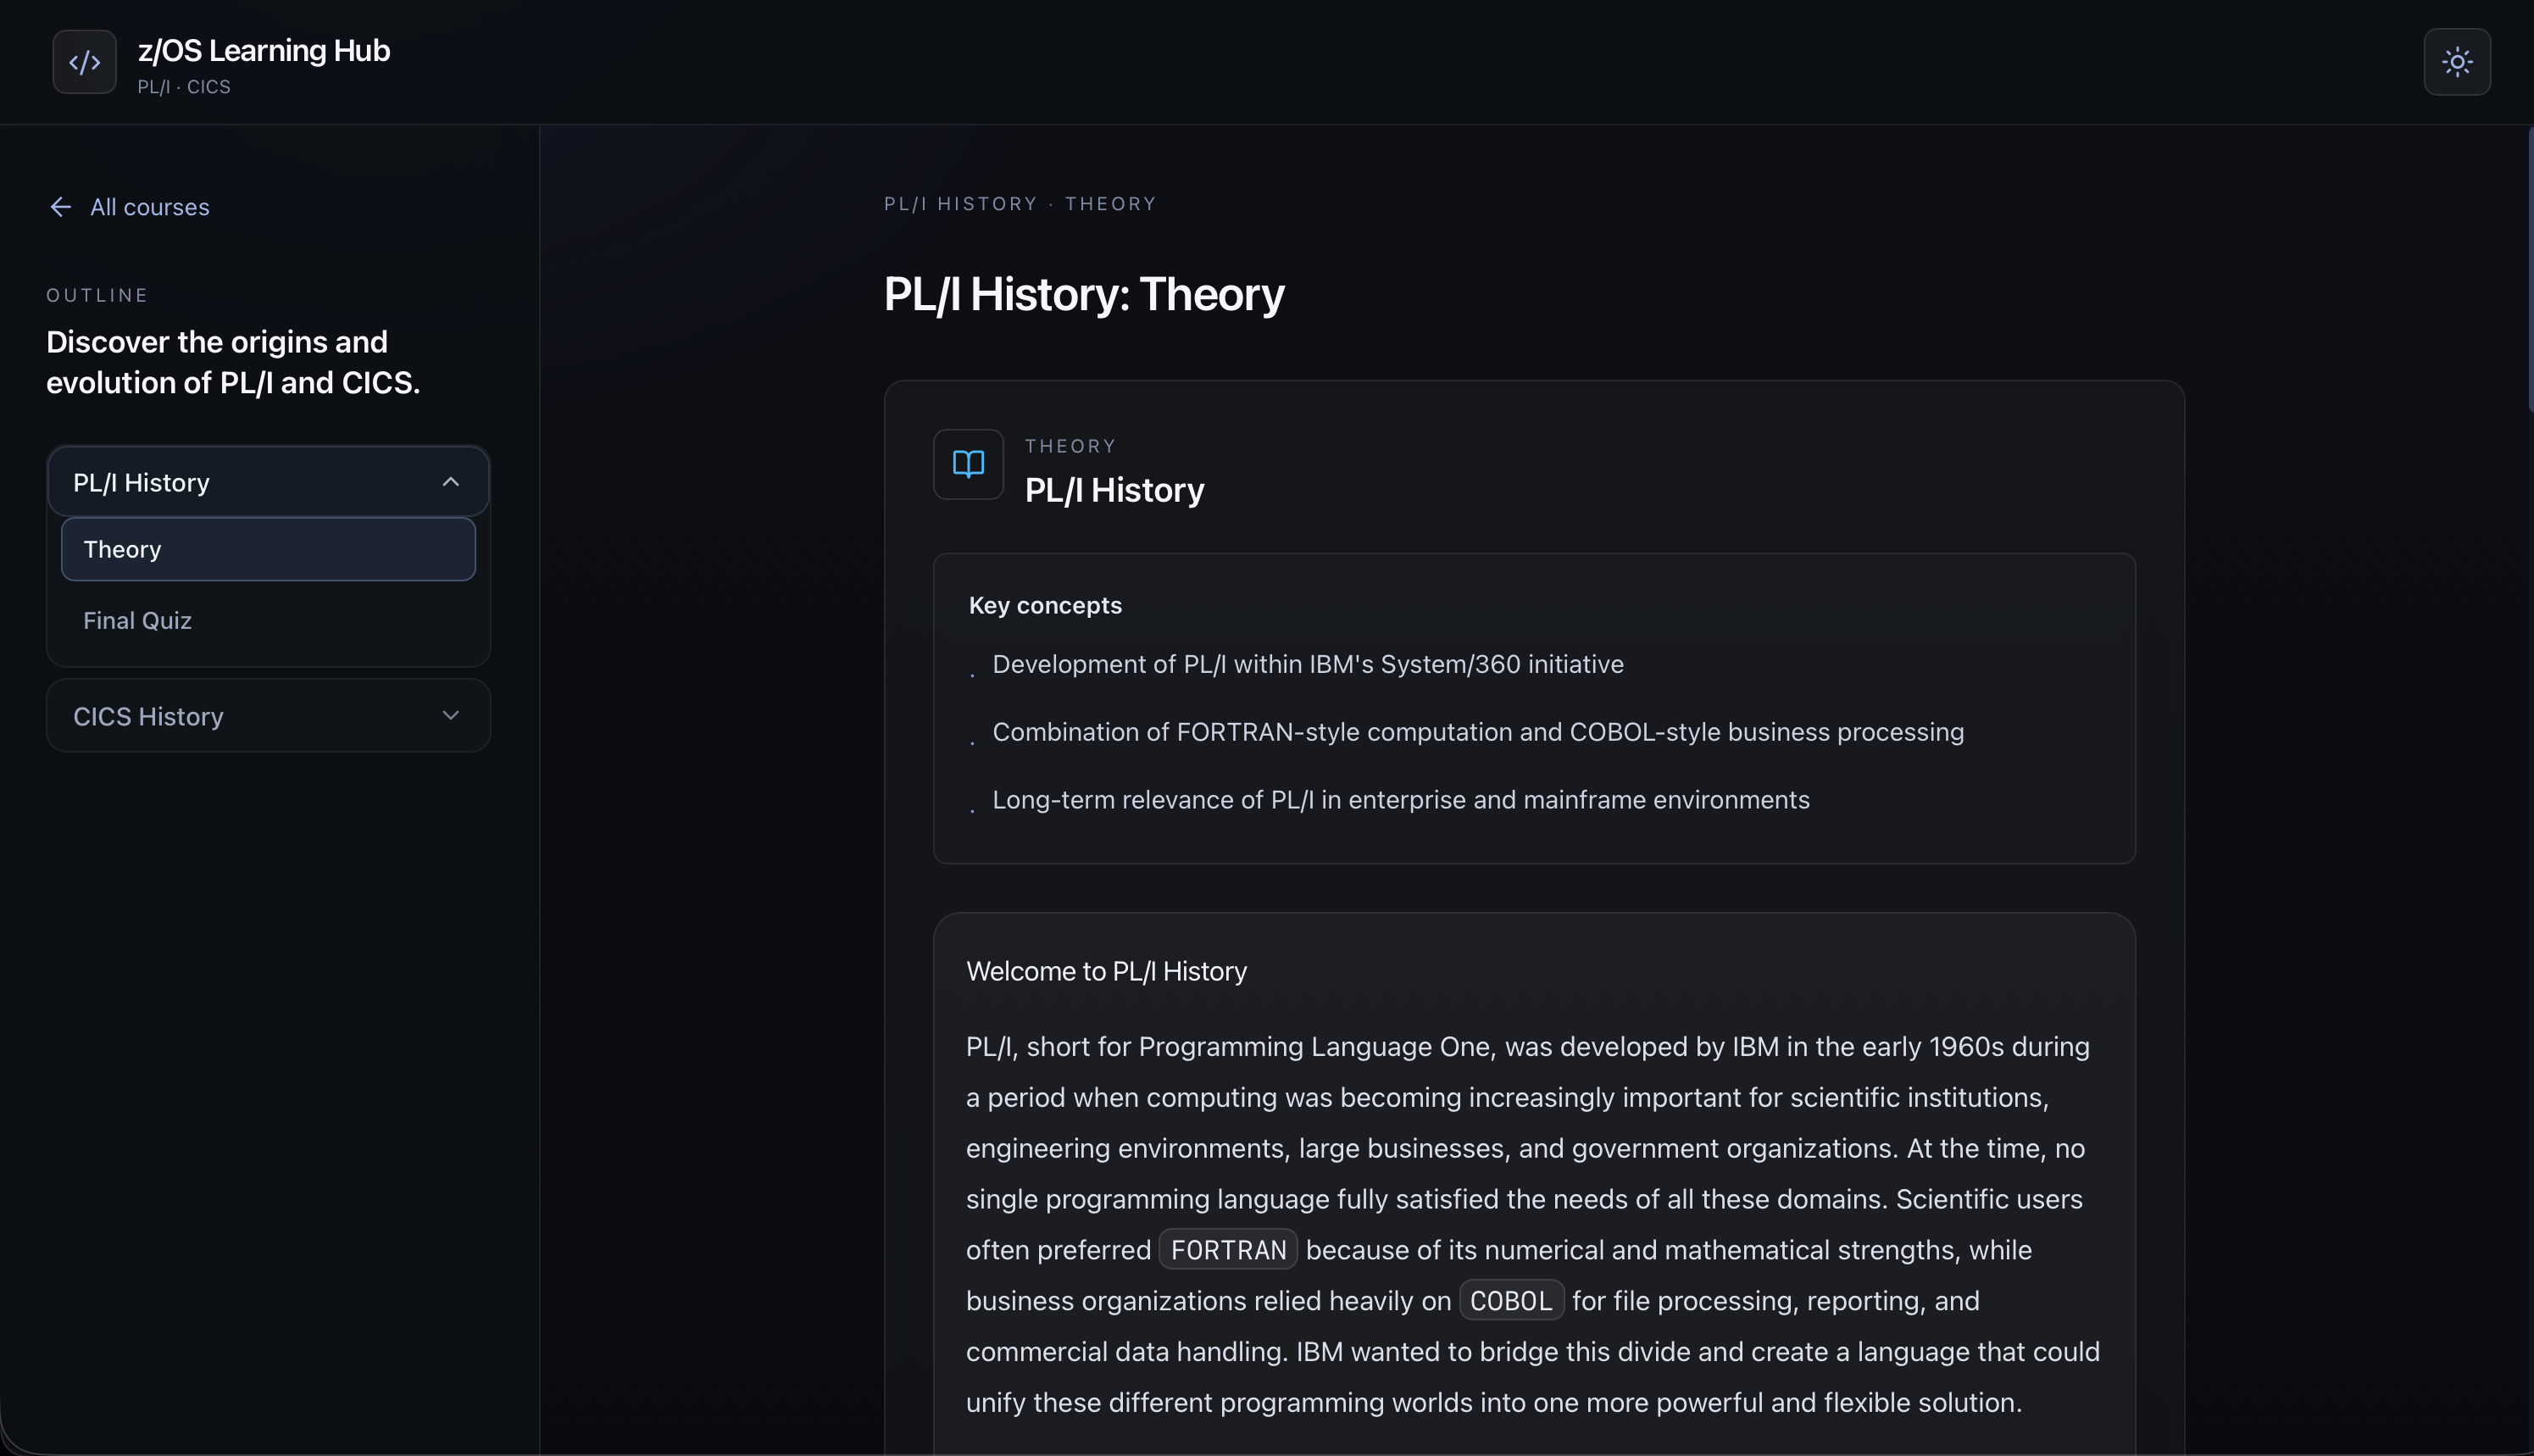
\includegraphics[width=0.8\textwidth]{../graphics/theorie.png}
   \caption[Theorie figuur.]{\label{fig:Theorie}Webite theorie module.}
 \end{figure}

Hier worden de kernconcepten en technische principes behandeld die noodzakelijk zijn om het onderwerp goed te begrijpen. 
De leerstof is gestructureerd opgebouwd waardoor studenten hun kennis kunnen opbouwen en verdiepen in onderwerpen die voorgaand werden besproken.
Hierdoor kan er eerst een brede basis worden aangebracht en later worden verdiept.
Dit is belangrijk omdat de materie binnen PL/I, CICS en mainframeontwikkeling vaak complex is en een sterke onderlinge samenhang vertoont.
Doordat de theorie op een logische manier en in fases wordt aangebracht kan de student een correct beeld krijgen van alle technologieën en hoe ze samenwerken.

Daarnaast wordt de theoretische uitleg aangevuld met concrete voorbeelden en extra bronnen.
Die voorbeelden helpen om abstracte concepten toegankelijker te maken en tonen hoe de theorie zich vertaalt naar praktische situaties.
De toegevoegde bronnen bieden studenten de mogelijkheid om zich verder te verdiepen in specifieke onderwerpen.
Ook kunnen ze aan de hand van deze bronnen de leerstof herbekijken wanneer iets niet helemaal duidelijk was.
Dit voorkomt dat de leersite een gesloten leeromgeving is, maar geeft studenten juist de mogelijkheid tot zelfstandig leren.
Studenten met meer interesse of voorkennis kunnen zich zo verder ontwikkelen terwijl anderen de basisinhoud op hun eigen tempo kunnen verwerken.

\subsection[short]{Oefeningen in modules}%
\label{sec:Oefeningen-module}

Na het theoretische gedeelte volgt het onderdeel met \textbf{de oefeningen}. 

\begin{figure}
   \centering
   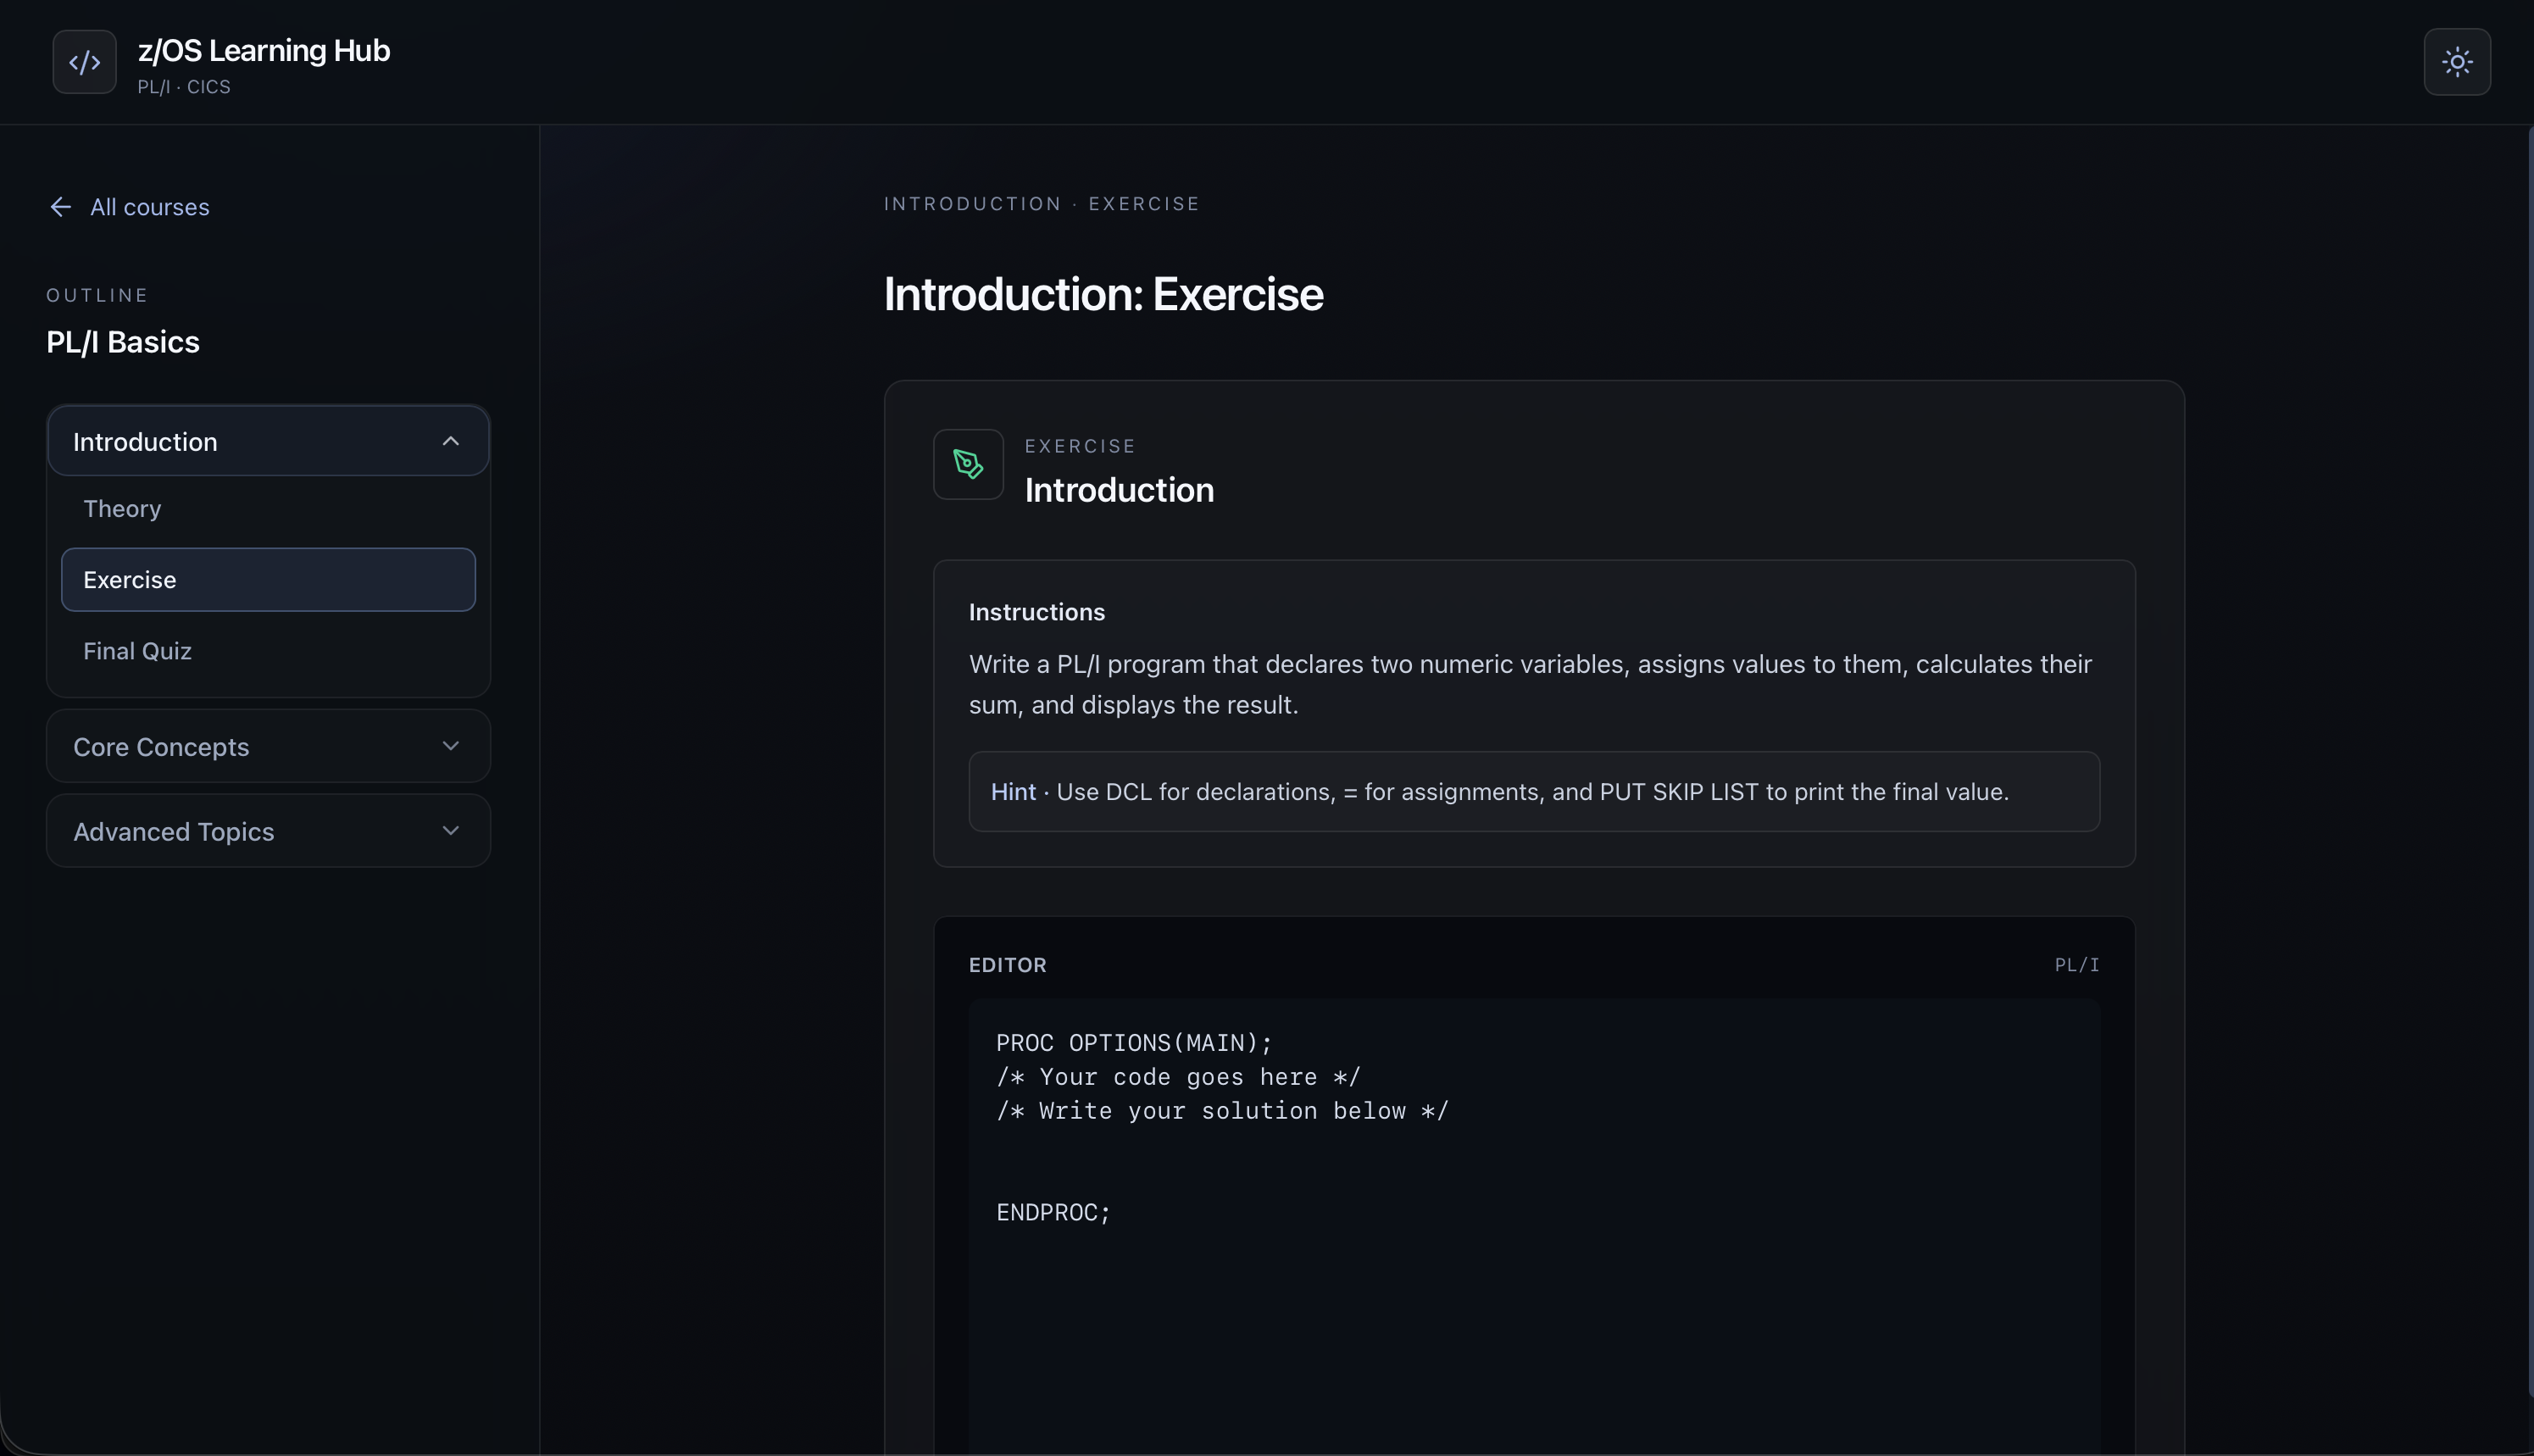
\includegraphics[width=0.8\textwidth]{../graphics/exercise.png}
   \caption[Oefeningen figuur.]{\label{fig:Oefeningen}Webite Oefeningen module.}
 \end{figure}

In deze fase wordt de student aangezet om de aangeleerde concepten toe te passen aan de hand van praktische voorbeelden.
De oefeningen sluiten rechtstreeks aan bij de inhoud die eerder in het hoofdstuk werd behandeld en vormen daardoor de verbinding tussen theorie en praktijk.
Dit onderdeel is essentieel, omdat technische kennis pas echt betekenis krijgt wanneer zij in de praktijk wordt gebruikt.

Door zelf programmeeroefeningen te maken en problemen op te lossen wordt de student gedwongen om actief na te denken over de leerstof in plaats van deze enkel passief op te nemen.
De oefeningen hebben daarbij niet uitsluitend een controlerende functie, maar maken deel uit van het leerproces.
Ze geven de gebruiker de mogelijkheid om te experimenteren en fouten te maken.
Hieruit kunnen ze inzicht krijgen in welke onderdelen reeds goed begrepen zijn en waar nog moeilijkheden liggen.
Vooral bij het leren programmeren is deze actieve verwerking van groot belang.

Vaardigheden zoals logisch redeneren, syntaxis correct toepassen en fouten herkennen worden immers niet alleen ontwikkeld door theorie te bestuderen, maar vooral door herhaaldelijk te oefenen.
De oefeningen zorgen er dus voor dat de leerstof niet oppervlakkig blijft maar effectief wordt omgezet in bruikbare vaardigheden.




\subsection[short]{Quiz in modules}%
\label{sec:Quiz-module}


Als afsluiting van elk hoofdstuk is er \textbf{een finale quiz} voorzien. 

\begin{figure}
   \centering
   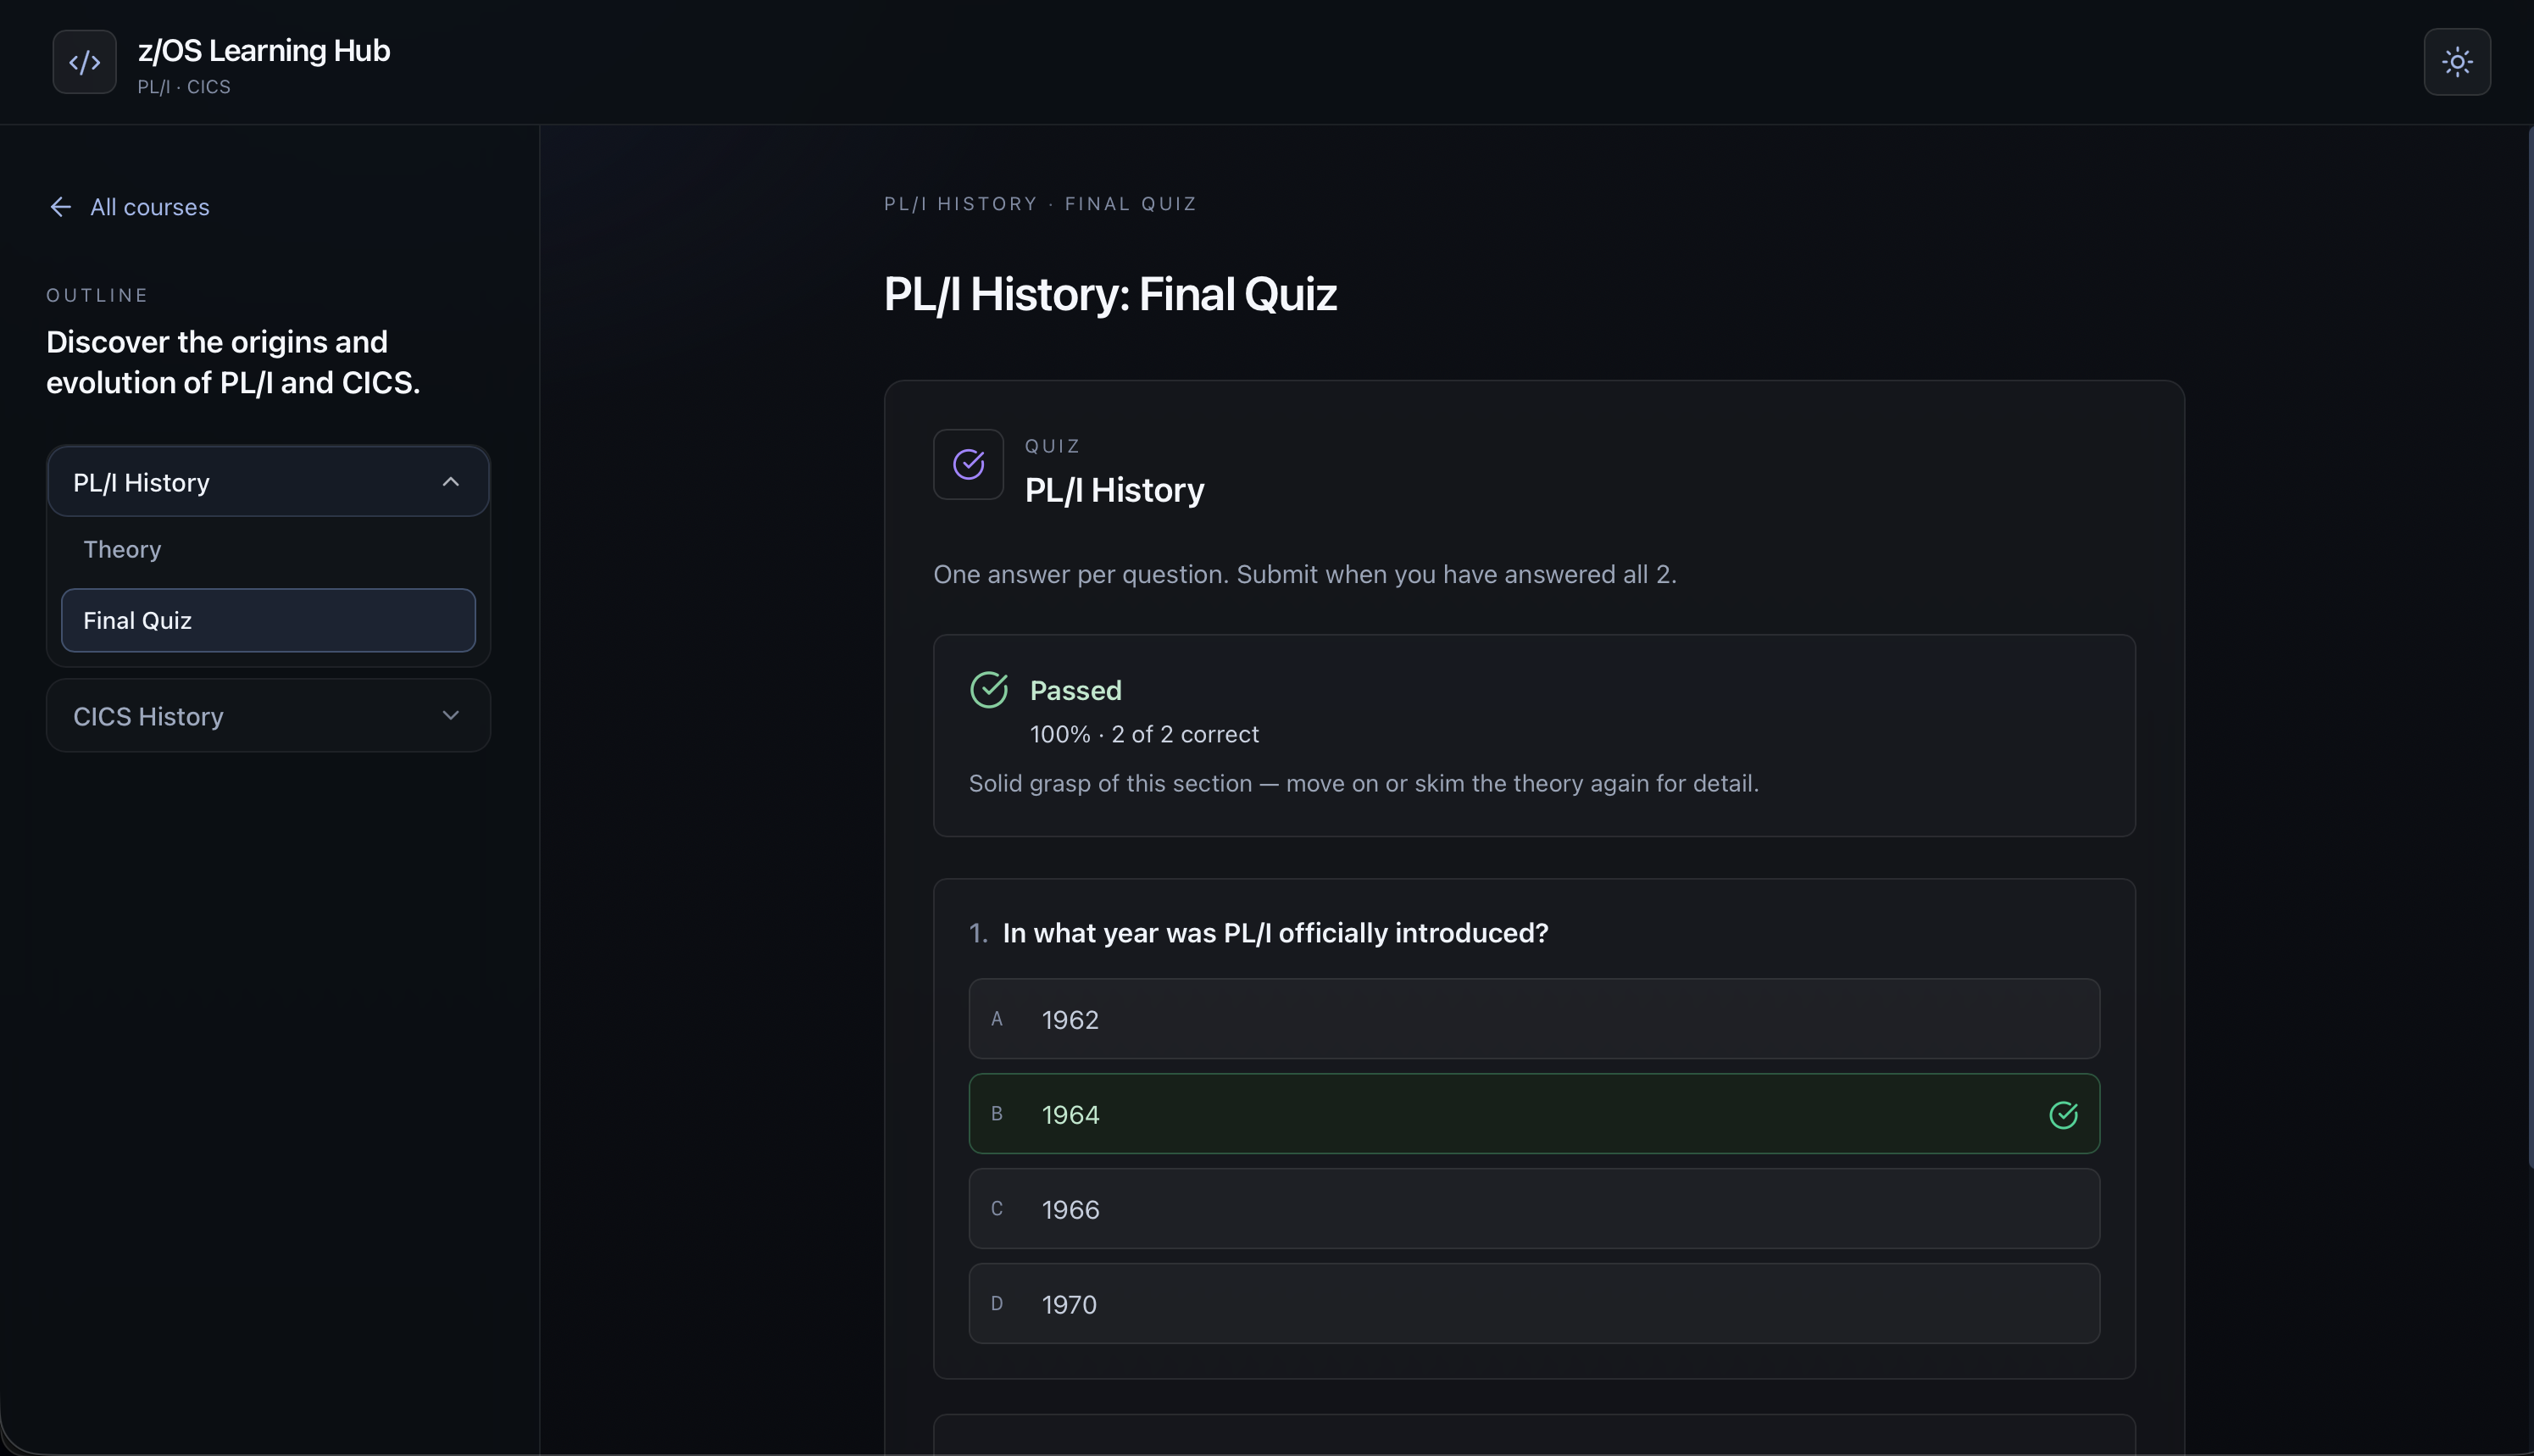
\includegraphics[width=0.8\textwidth]{../graphics/quiz.png}
   \caption[Quiz figuur.]{\label{fig:Quiz}Webite quiz module.}
 \end{figure}

Deze quiz heeft als doel om de volledige inhoud van het hoofdstuk te evalueren.
Waar de oefeningen zich eerder richten op het inoefenen van afzonderlijke onderdelen, brengt de quiz alle behandelde leerstof samen in één evaluatiemoment.

Hierdoor krijgt de student de kans om na te gaan of niet alleen de afzonderlijke concepten zijn begrepen maar ook het totaalbeeld duidelijk is.
Dit maakt de quiz tot een belangrijke tool om te kunnen meten in welke mate de leerstof van het hoofdstuk is verwerkt en opgenomen.

De finale quiz vervult bovendien een motiverende en structurerende rol binnen de leersite.
Ze biedt de student een duidelijk eindpunt van het hoofdstuk en stimuleert hen om de leerstof grondig door te nemen in plaats van ze enkel oppervlakkig te bekijken.
Ook maakt de quiz direct zichtbaar welke onderdelen al goed gekend zijn en welke nog verdere herhaling vereisen. 

Voor een online leersite is zo'n evaluatiemoment bijzonder waardevol om de student te helpen zelfstandig het eigen leerproces op te volgen.
De quiz vormt dus niet alleen een afsluitende test, maar ook een hulpmiddel om bewust en doelgericht verder te leren.


%

Door deze drie onderdelen in elk hoofdstuk te laten terugkeren, ontstaat een herkenbare en gestructureerde leeromgeving. 
De gebruiker weet telkens wat er verwacht wordt en doorloopt steeds dezelfde logische opbouw: eerst begrijpen, daarna toepassen, en tot slot evalueren. 
Die herhaling in de modulestructuur verhoogt de gebruiksvriendelijkheid van de leersite en ondersteunt het leerproces.
Het zorgt ervoor dat de focus niet ligt op het zoeken naar informatie of het navigeren door de inhoud, maar op het effectief verwerven van kennis. 
Zo draagt de gekozen opbouw rechtstreeks bij aan de academische kwaliteit en de praktische bruikbaarheid van de volledige leeromgeving.





